\documentclass[UTF8]{ctexart} 
%\usepackage{homework}
\usepackage{geometry}
\geometry{a4paper,scale=0.8}
\usepackage[table,xcdraw]{xcolor}
\usepackage{graphicx} %插入图片的宏包
\usepackage{float} %设置图片浮动位置的宏包
\usepackage{subfigure} %插入多图时用子图显示的宏包
\usepackage{enumerate}
%\usepackage{fancyhdr}  % header,footer的设置
%\usepackage{extramarks}
\usepackage{amsmath}  % 数学公式
\usepackage{amsthm}
\usepackage{amsfonts}
\usepackage{tikz}  % 绘图
\usepackage{algorithm}  % 算法
\usepackage{algorithmicx}
\usepackage{algpseudocode}  % 伪代码
%\usepackage[UTF8]{ctex}  % 支持中文
%\title{我的份}
%\author{randow}
%\begin{document}
%\maketitle
\title{
	
\includegraphics[scale = 1]{HDU.png}\\
    \vspace{1in}
    \textmd{ \Huge\textbf{机器学习}}\\
    \textmd{\textbf{神经网络调研学习报告}}\\
   	\vspace{3.5in}
	\textmd{19041822 罗汉东}\\
	\textmd{指导老师:朱素果}\\
%    \normalsize\vspace{0.1in}\small{\hmwkCompleteTime }\\
%    \vspace{0.1in}\large{\textit{\hmwkClassInstructor\ }}\\
}
%\usepackage{enumerate}
%\author{\hmwkAuthorName \\ 
%	\hmwkAuthorStuID}
%\date{}
\begin{document}
\maketitle
\newpage
\tableofcontents
\newpage
\section{人工神经网络(ANN)}
感知机是最简单的ANN架构,由Frank Rosenblatt于1957年发明。它基于被称作linear threshold unit (LTU)的人工神经元。LTU首先计算输入值的加权和$ (z=w_1x_1+w_2x_2+⋯+w_nx_n=W^T⋅X)$,然后对z应用一个阶梯函数(step function):

$$h_W(x)=step(z)=step(W^T⋅X)$$。
\begin{figure}[H]
\centering
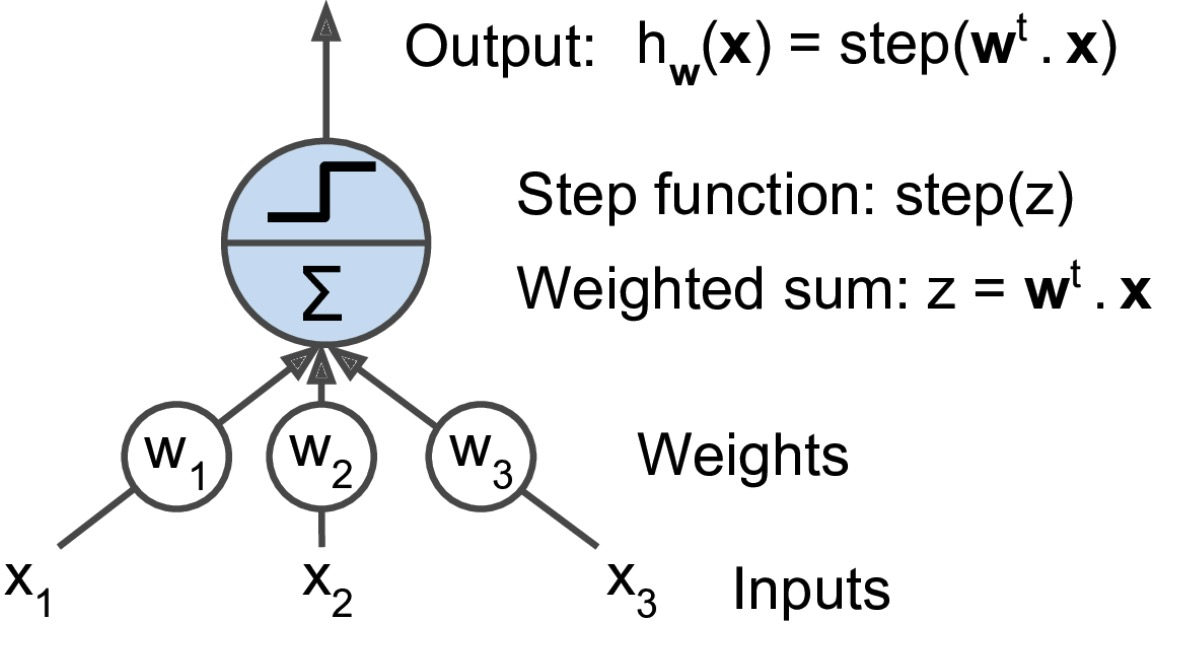
\includegraphics[scale = 0.4]{ANN.png}
\end{figure}
人工神经网络目前没有一个统一的正式定义。不过,具有下列特点的统计模型可以被称作是“神经化”的:
\begin{itemize}
    \item 具有一组可以被调节的权重(被学习算法调节的数值参数)
    \item 可以估计输入数据的非线性函数关系
\end{itemize}
这些可调节的权重可以被看做神经元之间的连接强度。

人工神经网络与生物神经网络的相似之处在于,它可以集体地、并行地计算函数的各个部分,而不需要描述每一个单元的特定任务。神经网络这个词一般指统计学、认知心理学和人工智能领域使用的模型,而控制中央神经系统的神经网络属于理论神经科学和计算神经科学。[1]

在神经网络的现代软件实现中,被生物学启发的那种方法已经很大程度上被抛弃了,取而代之的是基于统计学和信号处理的更加实用的方法。在一些软件系统中,神经网络或者神经网络的一部分(例如人工神经元)是大型系统中的一个部分。这些系统结合了适应性的和非适应性的元素。

虽然这种系统使用的这种更加普遍的方法更适宜解决现实中的问题,但是这和传统的连接主义人工智能已经没有什么关联了。不过它们还有一些共同点:非线性、分布式、并行化,局部性计算以及适应性。从历史的角度讲,神经网络模型的应用标志着二十世纪八十年代后期从高度符号化的人工智能(以用条件规则表达知识的专家系统为代表)向低符号化的机器学习(以用动力系统的参数表达知识为代表)的转变。

典型的人工神经网络具有以下三个部分:
\begin{description}
    \item[结构]结构指定了网络中的变量和它们的拓扑关系。例如,神经网络中的变量可以是神经元连接的权重(weights)和神经元的激励值(activities of the neurons)。
    \item[激励函数]大部分神经网络模型具有一个短时间尺度的动力学规则,来定义神经元如何根据其他神经元的活动来改变自己的激励值。一般激励函数依赖于网络中的权重(即该网络的参数)。
    \item[学习规则]  学习规则指定了网络中的权重如何随着时间推进而调整。这一般被看做是一种长时间尺度的动力学规则。一般情况下,学习规则依赖于神经元的激励值。它也可能依赖于监督者提供的目标值和当前权重的值。例如,用于手写识别的一个神经网络,有一组输入神经元。输入神经元会被输入图像的数据所激發。在激励值被加权并通过一个函数(由网络的设计者确定)后,这些神经元的激励值被传递到其他神经元。这个过程不断重复,直到输出神经元被激發。最后,输出神经元的激励值决定了识别出来的是哪个字母。
\end{description}
\section{卷积神经网络(CNN)}
卷积神经网络是一种前馈神经网络,它的人工神经元可以响应一部分覆盖范围内的周围单元,对于大型图像处理有出色表现。

卷积神经网络由一个或多个卷积层和顶端的全连通层(对应经典的神经网络)组成,同时也包括关联权重和池化层。这一结构使得卷积神经网络能够利用输入数据的二维结构。与其他深度学习结构相比,卷积神经网络在图像和语音识别方面能够给出更好的结果。

这一模型也可以使用反向传播算法进行训练。相比较其他深度、前馈神经网络,卷积神经网络需要考量的参数更少,使之成为一种颇具吸引力的深度学习结构。

CNN最重要的构件就是卷积层(卷积是一种数学运算,度量两个函数乘积的逐点积分。其与傅里叶变换与拉普拉斯变换高度相关,在信号处理中应用广泛。卷积层实际上使用了互相关,这与卷积是相似的。卷积处理的是连续变量,互相关好像是离散变量。):第一个卷积层的神经元并不和所有的输入全连接,只与其接受域的像素点连接。依次地,第二个卷积层也与第一个卷积层部分相连。这一架构使得第一个隐层专注于低级别特征,然后在随后的隐层中将低级别特征进行组合。

\section{循环神经网络(RNN)}
循环神经网络是神經網絡的一種。单纯的RNN因为无法处理随着递归,权重指数级爆炸或梯度消失问题,难以捕捉长期时间关联;而结合不同的LSTM可以很好解决这个问题。

时间循环神经网络可以描述动态时间行为,因为和前馈神经网络接受较特定结构的输入不同,RNN将状态在自身网络中循环传递,因此可以接受更广泛的时间序列结构输入。手写识别是最早成功利用RNN的研究结果。

基本的 RNN 是由人工神经元组织成的连续的层的网络。给定层中的每个节点都通过有向(单向)连接连接到下一个连续层中的每个其他节点。每个节点(神经元)都有一个时变的实值激活。每个连接(突触)都有一个可修改的实值权重。节点要么是输入节点(从网络外部接收数据),要么是输出节点(产生结果),要么是隐藏节点(在从输入到输出的过程中修改数据)。

对于离散时间设置中的监督学习,实值输入向量序列到达输入节点,一次一个向量。在任何给定的时间步长,每个非输入单元将其当前激活(结果)计算为与其连接的所有单元的激活的加权和的非线性函数。可以在特定的时间步长为某些输出单元提供主管给定的目标激活。例如,如果输入序列是对应于口语数字的语音信号,则在序列末尾的最终目标输出可以是对该数字进行分类的标签。

在强化学习环境中,没有教师提供目标信号。相反,适应度函数或奖励函数偶尔用于评估RNN的性能,它通过影响输出单元来影响其输入流,输出单元和一个可以影响环境的执行器相连。这可以被用来玩一个游戏,在这个游戏中,进度是用赢得的点数来衡量的。

每个序列产生一个误差,作为所有目标信号与网络计算的相应激活的偏差之和。对于大量序列的训练集,总误差是所有单个序列误差的总和。

Elman网络是一个三层网络,添加了一组上下文单元。中间(隐藏)层连接到这些权重为1的上下文单元。在每个时间步,输入被向前反馈,并且学习规则被应用。固定的反向连接在上下文单元中保存隐藏单元的先前值的副本(因为它们在应用学习规则之前在连接上传播)。因此,网络可以保持某种状态,允许它执行诸如序列预测之类的任务,这些任务超出了标准多层感知器的能力。

Jordan网络类似于Elman网络。上下文单元是从输出层而不是隐藏层馈送的。Jordan网络中的上下文单元也称为状态层。他们与自己有着经常性的联系。

Elman和Jordan网络也被称为“简单循环网络”。
\section{BP神经网络}
BP是“误差反向传播”的简称,是一种与最优化方法(如梯度下降法)结合使用的,用来训练人工神经网络的常见方法。该方法对网络中所有权重计算损失函数的梯度。这个梯度会回馈给最佳化方法,用来更新权值以最小化损失函数。

任何监督式学习算法的目标是找到一个能把一组输入最好地映射到其正确的输出的函数。例如一个简单的分类任务,其中输入是动物的图像,正确的输出将是动物的名称。一些输入和输出模式可以很容易地通过单层神经网络(如感知器)学习。但是这些单层的感知机只能学习一些比较简单的模式,例如那些非线性可分的模式。

例如,人可以通过识别动物的图像的某些特征进行分类,例如肢的数目,皮肤的纹理(无论是毛皮,羽毛,鳞片等),该动物的体型,以及种种其他特征。但是,单层神经网络必须仅仅使用图像中的像素的强度来学习一个输出一个标签函数。因为它被限制为仅具有一个层,所以没有办法从输入中学习到任何抽象特征。多层的网络克服了这一限制,因为它可以创建内部表示,并在每一层学习不同的特征。

第一层可能负责从图像的单个像素的输入学习线条的走向。第二层可能就会结合第一层所学并学习识别简单形状(如圆形)。每升高一层就学习越来越多的抽象特征,如上文提到的用来图像分类。每一层都是从它下方的层中找到模式,就是这种能力创建了独立于为多层网络提供能量的外界输入的内部表达形式。 反向传播算法的发展的目标和动机是找到一种训练的多层神经网络的方法,于是它可以学习合适的内部表达来让它学习任意的输入到输出的映射。

反向传播要求有对每个输入值想得到的已知输出,来计算损失函数梯度。因此,它通常被认为是一种監督式學習方法,虽然它也用在一些无监督网络(如自动编码器)中。

它是多层前馈网络的Delta规则的推广,可以用链式法则对每层迭代计算梯度。反向传播要求人工神经元(或“节点”)的激励函数可微。

BP神经网络是一种多层的前馈神经网络,其主要的特点是:信号是前向传播的,而误差是反向传播的。具体来说,对于如下的只含一个隐层的神经网络模型:

BP神经网络的过程主要分为两个阶段,第一阶段是信号的前向传播,从输入层经过隐含层,最后到达输出层;第二阶段是误差的反向传播,从输出层到隐含层,最后到输入层,依次调节隐含层到输出层的权重和偏置,输入层到隐含层的权重和偏置。

BP网络采用的传递函数是非线性变换函数——Sigmoid函数(又称S函数)。其特点是函数本身及其导数都是连续的,因而在处理上十分方便。为什么要选择这个函数,等下在介绍BP网络的学习算法的时候会进行进一步的介绍。S函数有单极性S型函数和双极性S型函数两种,单极性S型函数定义如下:$f(x)=\frac{1}{1+e^{−x}}$,双极性S型函数定义如下:$f(x)=\frac{2}{1+e^{−x}}-1$。

使用S型激活函数时,输入:$$net=x_1w_1+x_2w_2+...+x_nw_n$$

输出:$$ y=f(net)=\frac{1}{1+e^{-net}}$$
    
输出的导数:$$f^{'}(net)=\frac{1}{1+e^{-net}}-\frac{1}{(1+e^{-net})^2}=y(1-y)$$

\section{残差神经网络}
对于传统的深度学习网络应用来说,网络越深,所能学到的东西越多。当然收敛速度也就越慢,训练时间越长,然而深度到了一定程度之后就会发现越往深学习率越低的情况,甚至在一些场景下,网络层数越深反而降低了准确率,而且很容易出现梯度消失和梯度爆炸。

这种现象并不是由于过拟合导致的,过拟合是在训练集中把模型训练的太好,但是在新的数据中表现却不尽人意的情况。从上图可以看出,我们的训练准误差和测试误差在层数增加后皆变大了,这说明当网络层数变深后,深度网络变得难以训练。

网络太深,模型就会变得不敏感,不同的图片类别产生了近似的对网络的刺激效果,这时候网络均方误差的减小导致最后分类的效果往往不会太好,所以解决思路就是引入这些相似刺激的“差异性因子”。

​深度残差网络(ResNet)的设计就是为了克服这种由于网络深度的加深而产生的学习率变低、准确率无法有效提升的问题。

引入“捷径”,可以防止梯度消失问题,其实在ResNet出来以前已经有人对这方面进行研究了,Srivastava等人的“公路网络”,“培训非常深的网络”是类似的方法,他们认为更深层的网络应该也是易于优化的,层数越多准确率越高,训练方法与“传统”深度网络相比不会有很大变化

对于跳跃结构,当输入与输出的维度一样时,不需要做其他处理,两者相加就可,但当两者维度不同时,输入要进行变换以后去匹配输出的维度,主要经过两种方式
\begin{enumerate}
    \item 用zero-padding去增加维度
    \item 用1x1卷积来增加维度
\end{enumerate}

  普通的神经网络,随着网络深度的加深,训练错误会越来越多。但有了ResNets就不一样了,即使网络再深,训练的表现却不错,比如说训练误差减少,这种方式确实有助于解决梯度消失和梯度爆炸问题,让我们在训练更深网络的同时,又能保证良好的性能。
\end{document}